\section{Versuchsauswertung}

\subsection{Eloxieren}
\begin{longtable}{p{3cm}p{14cm}}
    \textbf{Beizen}
    & Nach dem Eintauchen in die Natronlauge hat wie erwartet sofort eine starke \chemfig{H_2}-Bildung eingesetzt. Dabei wurde die Passivoxidschicht des Aluminiums entfernt und gleichzeitig die Oberfläche angeätzt. Die Luft begann stark ätzend zu riechen, was wahrscheinlich auf das Herausspritzen von winzigen \chemfig{NaOH}-Partikeln zurückzuführen ist.\\
    \hline
    
    \textbf{Eloxieren}
    & Nach dem Zwischenspülen wurden die Gemüseschäler für eine Stunde in die Schwefelsäure getaucht. Dabei mussten wir zwischenzeitlich immer wieder die beiden Aluelektroden auf den Kontaktstäben hin- und herbewegen, da sie teilweise nicht mehr guten Kontakt gemacht haben. Für das Eloxieren ist jedoch ein gleichmässiger Fluss des Stromes von beiden Seiten notwendig damit die Eloxalschicht überall gleichmässig dick wird.\newline
    Der benötigte Strom für das Eloxieren wurde wie folgt durch geschätzte Flächen berechnet:\\
    &     $$\begin{aligned}
            S_{Handgriff} &= 0.612 dm^2\\
            S_{Verbindung} &= 0.063 dm^2\\
            S_{gesamt} &= 0.675 dm^2\\
            S_{Referenz} &= 0.5 dm^2\\
            \\
            I_{Elox} = J\cdot A &= 1.4 A/dm^2 \cdot (2\cdot S_{gesamt} + S_{Referenz}) = 2.59 A
            \end{aligned}$$\\
    \hline
    
    \textbf{Einf\"arben}
    & Das Färben verlief wie erwartet problemlos. Die Gemüseschäler wurden für fünf Minuten in die 60 Grad heisse Farbe getaucht.\\
    & Die hohe Temperatur wird gewählt, damit das thermische Schwingen höher ist und somit die Farbpartikel auch besser in die Poren der Eloxalschicht eindringen können.\\
    \hline
    
    \textbf{Verdichten}
    & Um die Poren der Eloxalschicht zu schliessen wurden die Gemüseschäler für 45 Minuten in kochendes deionisiertes Wasser gelegt. Dabei wurde das Aluminiumhydroxid mit Wasser angereichert und dieses wurde anschliessend zu Böhmit umgewandelt, welcher ein grösseres Volumen beansprucht und damit die Poren verschliesst.\\
    \hline
    
    \textbf{Schichtdicken-bestimmung}
    & Zur Bestimmung der Eloxal-Schichtdicke wurde das Referenzaluplättchen nach dem Eloxieren zuerst getrocknet und anschliessend mit einer Präzisionswaage gewogen. Die Masse betrug: $$ m_1 = 9.86728 \mathrm{g}$$
    Danach wurde dieses Plättchen für rund 15 Minuten in kochende Chrom-Phosphorsäure gelegt. Dadurch wurde die Eloxalschicht entfernt, das Aluminium selber jedoch nicht angegriffen. Das Gewicht der Passivoxidschicht, welche sofort wieder entsteht sobald das Aluminium mit Sauerstoff in Kontakt kommt, kann vernachlässigt werden. Das nach erneutem Trocknen gemessene Gewicht des Plättchen betrug: $$ m_2 = 9.63671 \mathrm{g}$$
    Berechnung der Schichtdicke:
    $$ \begin{aligned}
            m_{Eloxalschicht} &= m_1 - m_2 = 0.23057 \mathrm{g}\\
            \rho_{Eloxal} &= 2.5\cdot 10^{6} \frac{\mathrm{g}}{\mathrm{m}^3} \qquad \text{(unverdichtet)}\\
            V_{Eloxal} &= \frac{m_{Eloxalschicht}}{\rho_{Eloxal}} = \frac{0.23057 \mathrm{g}}{2.5\cdot 10^{6} \frac{\mathrm{g}}{\mathrm{m}^3}} = 92.228 \cdot 10^{-9} \mathrm{m^3}\\
            S_{Referenz} &= 5 \cdot 10^{-3} \mathrm{m^2}\\
            d_{Eloxal} &= \frac{V_{Eloxal}}{S_{Referenz}} = \frac{92.228 \cdot 10^{-9} \mathrm{m^3}}{5 \cdot 10^{-3} \mathrm{m^2}}= 18.45 \mathrm{\mu m}
       \end{aligned}$$\\
    & Gemäss Abbildung 2 Seite 4 des Versuchsskriptes sollte die Eloxalschichtdicke nach 45 Minuten eloxieren ungefähr $20 \mathrm{\mu m}$ betragen. Somit stimmt die von uns durch die Massendifferenz berechnete Schichtdicke von $18.45 \mathrm{\mu m}$ relativ gut überein.\\
    \hline
\end{longtable}

\subsection{Galvanisieren}
\begin{longtable}{p{3cm}p{14cm}}
    \textbf{Oberfläche}
    & Wir haben zwei 5-Liber und zwei verschiedene Schlüssel galvanisiert. Die Oberflächen der verschiedenen Werkstücken betrugen:
    $$\begin{aligned}
        S_{Schluessel\, 1} &= 1.732 \cdot 10^{-3} \mathrm{m^2}\\
        S_{Schluessel\, 2} &= 1.263 \cdot 10^{-3} \mathrm{m^2}\\
        S_{5-Liber} &= 1.753 \cdot 10^{-3} \mathrm{m^2}\\
        S_{gesamt} &= 6.501 \cdot 10^{-3} \mathrm{m^2}
    \end{aligned}$$\\
    \hline
    
    \textbf{Elektrolytisches Entfetten}
    & Unsere Metallproben wurden für ca. 45 Sekunden bei einem Strom von 5A ins \chemfig{NaOH}-Bad getaucht. Dies war der vom Netzteil maximal lieferbare Strom. Dabei haben sich Schmutzpartikel, welche vorher durch das Ultraschallbad und die Handreinigung nicht entfernt wurden, gelöst und sind durch die \chemfig{H_2}-Bildung und der im Bad enthaltenden Emulsion an die Oberfläche getragen worden.\\
    \hline
    
    \textbf{Dekapieren}
    & Während dem Dekapieren hat man absolut nichts gesehen. Es entstand keine Blasenbildung. Es wurde lediglich der Oxidschichtfilm auf unseren Metallproben entfernt.\\
    \hline
    
    \textbf{Verkupfern}
    & Stromberechnung für das Verkupfern:
    $$\begin{aligned}
        J &= 100 \mathrm{A/m^2}\\
        I_{berechnet} &= J \cdot S_{gesamt} = 650 \mathrm{mA}
    \end{aligned}$$
    
    Wir haben die Spannung vor dem Eintauchen nicht ganz auf 4V eingestellt. Sobald aber die Werkstücke in die Lösung getaucht waren, haben wir den berechneten Strom eingestellt. Der ganze Vorgang dauerte 10 Sekunden. Es entstanden keine Probleme beim Verkupfern.\\
    \hline
    
    \textbf{Vernickeln}
    & Stromberechnung für das Vernickeln:
    $$\begin{aligned}
        J &= 500 \mathrm{A/m^2}\\
        I_{berechnet} &= J \cdot S_{gesamt} = 3.25 \mathrm{A}
    \end{aligned}$$
    
    Beim Vernickeln war es wichtig, dass die Spannung von 2V nicht überschritten wurde. Es wurde also nicht die vorher berechnete Stromstärke vollständig erreicht. Während dem Vernickeln ist aber der Strom dann kontinuierlich etwas angestiegen. Wir haben mit einer Konstantspannung von 1.9V vernickelt. Nach 8 Minuten haben wir die Werkstücke aus der Lösung entfernt und gewässert. Der Vorgang verlief ebenfalls problemlos.\\
    \hline
    
    \textbf{Vergolden}
    & Stromberechnung für das Vergolden:
    $$\begin{aligned}
        J &= 45 \mathrm{A/m^2}\\
        I_{berechnet} &= J \cdot S_{gesamt} = 30 \mathrm{mA}
    \end{aligned}$$
    
    Der berechnete Strom kam uns von Anfang an sehr klein vor. Dies hat sich nach der 2-minütigen Vergoldungszeit auch so gezeigt. Denn es wurde während dieser Zeit kein Gold abgeschieden. Die Oberflächen der Werkstücke sahen aus wie vorher. Grund dafür könnte sein, dass das neue Goldbad ganz andere Parameter hat als im Versuchsskript beschrieben. Denn auch die Vergoldungszeit war ja nur 2 Minuten anstatt 7 Minuten. Wahrscheinlich ist die Stromdichte von 45 $\mathrm{A/m^2}$ zu klein bei einer Vergoldungszeit von nur 2 Minuten.\newline
    In einem zweiten Durchgang haben wir die Stromstärke dann auf ca. 290mA erhöht. Dieser zweite Durchgang dauerte 1 Minute. Da während der ersten Phase sichtbar kein Gold abgeschieden wurde, haben wir dies nicht in die Berechnung der Goldmenge hineingenommen.\newline
    Um die abgeschiedene Goldmenge zu berechnen, muss man beachten, dass nicht der gesamte Strom in die Goldabscheidung hineinfliesst, sondern dass auch ein Teil in die Zersetzung von Wasser geht.
\end{longtable}
\newpage

\begin{longtable}{p{3cm}p{14cm}}
    & Berechnung der effektiven Stromdichte:
    $$\begin{aligned}
        I_{gemessen} &= 0.29 A\\
        J_{gemessen} &= \frac{I_{gemessen}}{S_{gesamt}} = \frac{0.29 A}{6.501 \cdot 10^{-3} \mathrm{m^2}} = 44.6 \mathrm{A/m^2} = 0.45 \mathrm{A/dm^2}
    \end{aligned}$$
    Mit der nun berechneten Stromdichte von 0.45 $\mathrm{A/dm^2}$ geht man nun in die folgende Grafik und kann ablesen, dass ca. 0.36 $\mathrm{A/dm^2}$ dieser Stromdichte für die Abscheidung von Gold zuständig waren.
\end{longtable}
\begin{figure}[H]\centering
    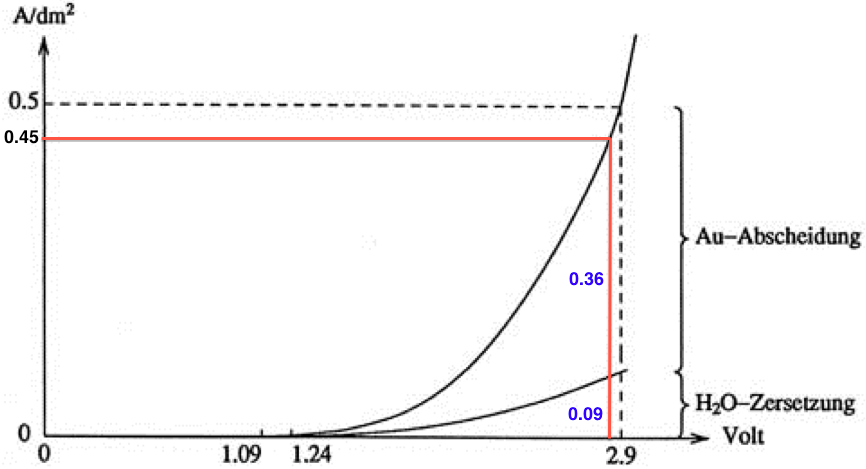
\includegraphics[width=10cm]{./pictures/AuAbscheidung.png}\\
    \caption{Zersetzungsspannungen beim Vergolden}
\end{figure}

\begin{longtable}{p{3cm}p{14cm}}
    & Somit errechnet sich der Strom, der für die Goldabscheidung zuständig war und die dabei abgeschiedene Goldmenge:
    $$\begin{aligned}
        I_{Au} &= J_{Au} \cdot S_{gesamt} = 36 \mathrm{A/m^2} \cdot 6.501 \cdot 10^{-3} \mathrm{m^2} = 234 \mathrm{mA}\\
        m_{Au} &= \frac{M \cdot I_{Au} \cdot t}{F} = \frac{196.97 \cdot 10^{-3} \frac{\mathrm{kg}}{\mathrm{mol}} \cdot 0.234 A \cdot 60 s}{96'500 \frac{\mathrm{C}}{\mathrm{mol}}} = 28.66 \mathrm{\mu g}\\
        d_{Au} &= \frac{m_{Au}}{\rho_{Au} \cdot S_{gesamt}} = \frac{28.66 \cdot 10^{-6} \mathrm{kg}}{19.32 \cdot 10^3 \mathrm{kg/m^3} \cdot 6.501 \cdot 10^{-3} \mathrm{m^2}} = 228 \mathrm{nm}
    \end{aligned}$$
    Bei einem Goldpreis von 25'000 Fr./kg entspricht dies in ungefähr Gold im Wert von:
    $$\begin{aligned}
        Preis &= 228 \cdot 10^{-9} \mathrm{kg} \cdot 25'000 \mathrm{Fr./kg} = 5.7 \cdot 10^{-3} \mathrm{Fr.} = 0.57 \mathrm{Rp.}
    \end{aligned}$$\\
    
    & Im Allgemeinen hat auch das Vergolden gut funktioniert. Einzig bei einem Fünflieber gab es eine kleine Auflagefläche, wo dementsprechend nicht vergoldet wurde. Die aufgetragene Goldmasse beträgt nun also 28.66 $\mathrm{\mu g}$, die Goldschichtdicke beträgt 228 nm und der Wert dieses Goldes 0.57 Rappen.
    
\end{longtable}